\section{Introduction}
\noindent Video inpainting targets to recover the missing contents of given videos, which can assist lots of practical applications, e.g., video restoration and augmented reality. Compared with image inpainting, video inpainting is much more challenging due to extra time dimension. It requires not only reasonable spatial structures but also stable temporal consistency. Specifically, directly applying 2D image inpainting algorithm \cite{yu2018free,Xiong_2019_CVPR} to individual frames is a sub-optimal choice, due to serious artificial effect, flickers and jitters. 

To exploit complementary neighbor information across frames, traditional patch-based methods \cite{patwardhan2007video,wexler2004space,newson2014video} recurrently copy the similar patches from unmasked regions and past them to the missing regions. 
\begin{figure}[t]
	\centering
	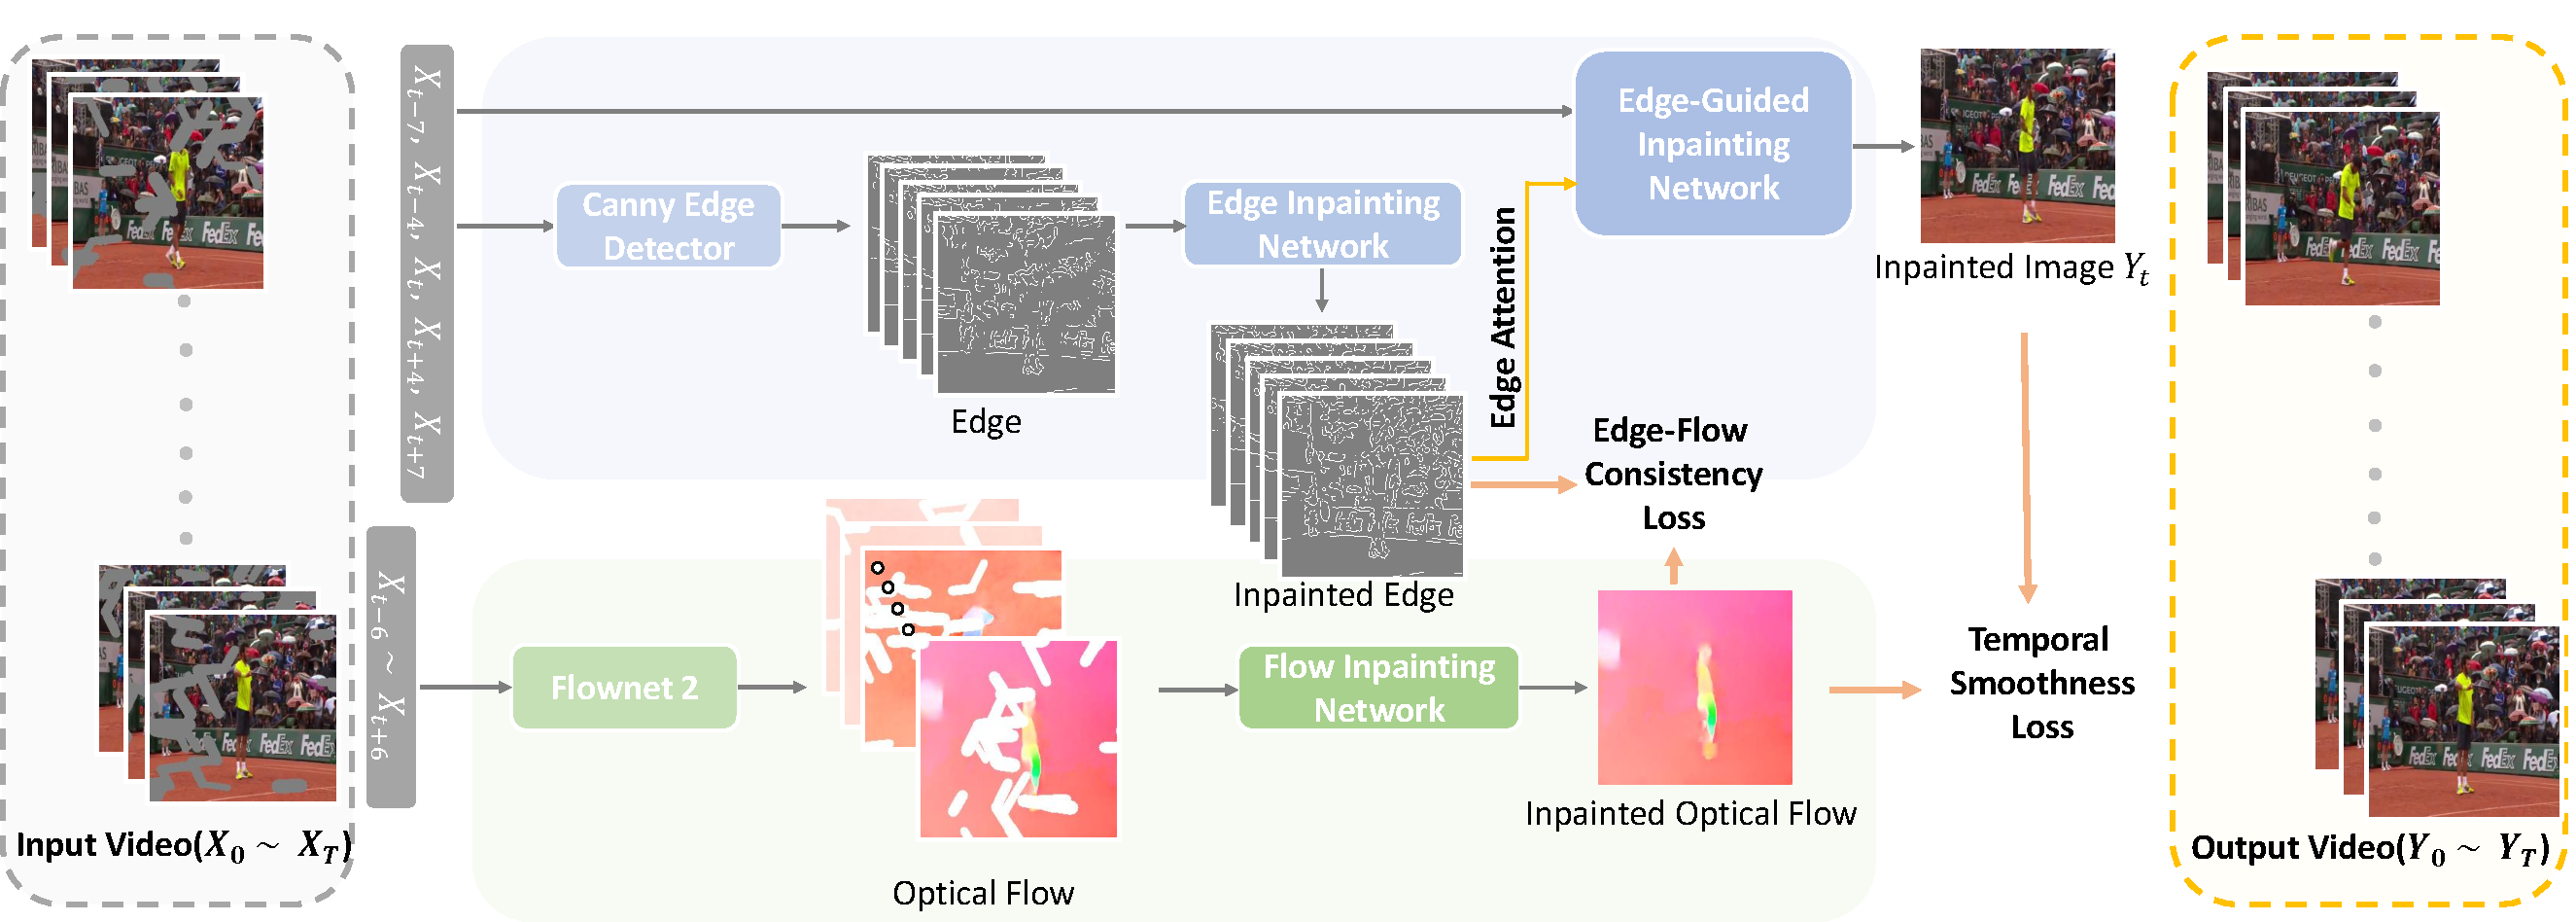
\includegraphics[width=1.0\columnwidth]{zong} % Reduce the figure size so that it is slightly narrower than the column. Don't use precise values for figure width.This setup will avoid overfull boxes. 
	\caption{The overall pipeline of STSENet. The ENet and FNet first complete the missing edge and optical flow across frames. Then, under the guidance of auxiliary edge and optical flow, STI can produce structure-preserved and temporally consistent inpainting frame.}
	\label{zong}
\end{figure}
This kind of methods depends on a strong hypothesis that the missing content have appeared in neighboring frames, which limits their generalization.
Recently, deep-learning based methods achieve state-of-the-art performance by treating a video as volume.
They utilize the CNNs, e.g., 3D convolution operation \cite{wang2019video}, to predict missing content with smooth motion, which is learned from training data.
Among these methods, optical flow is commonly used to temporally smooth contents \cite{Xu_2019_CVPR,Kim_2019_CVPR,Kim_2019_CVPR1} by aggregating contextual information.
However, the auxiliary motion compensation brought by optical flow lacks detailed structural clues.
Specifically, the inner textures of objects in optical flow are usually missed, leading to deficient structure rationality.
Thus, it is difficult to obtain both temporal consistent and structure-preserved inpainting video, by only using optical flow.





\begin{figure*}[t]
	\centering
	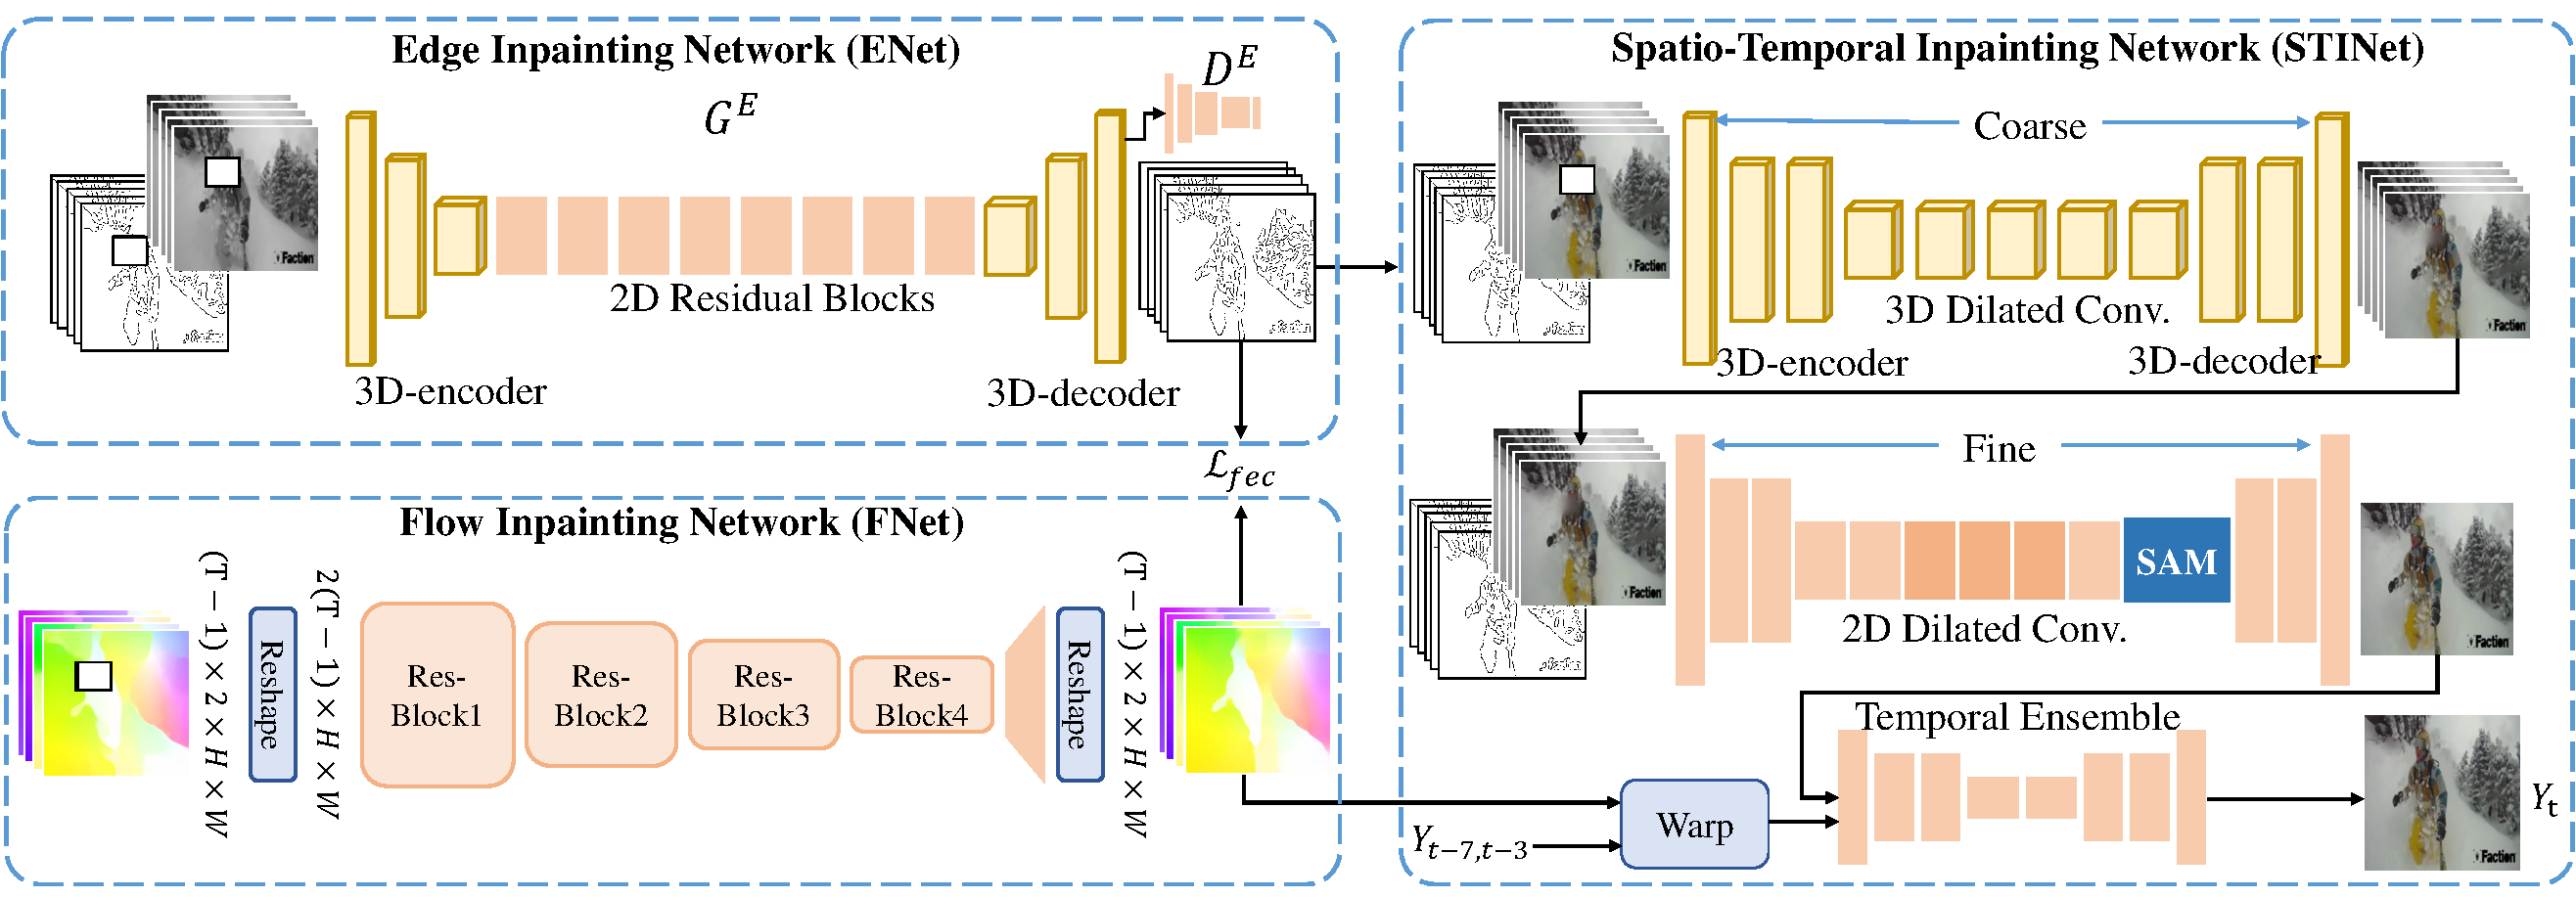
\includegraphics[width=2.0\columnwidth]{sti} % Reduce the figure size so that it is slightly narrower than the column. Don't use precise values for figure width.This setup will avoid overfull boxes. 
	\caption{The detailed architecture of STSENet. ENet adopts an encoder-decoder architectures with both 3D and 2D convolutions. FNet uses the Resnet101 as backbone, followed by a decoder. STI inpaints the frames in a coarse-to-fine manner. In FNet, $T$ is the number of input frames, and channel $2$ denotes the motion along $x$ and $y$ axis. To save space, all the input masks are omitted.}
	\label{fig:stiNet}
\end{figure*}
To address above issues, we present a novel video inpainting network, called Spatio-Temporal Structure Enhancement Network (STSENet), by simultaneously exploring optical flow and structural clues, to eliminate temporal flickers and enhance spatial detail. 
As shown in Fig.~\ref{zong}, STSENet consists of three modules, which are the ENet, FNet, and STI, respectively.
Given frames with missing pixels, ENet and FNet first predict the missing edge and optical flow, which indicate the structure knowledge and motion tendency.
%according to learned structure knowledge and motion tendency from the training data,
Instead of separate training, these two modules are associated with each other via a flow-edge consistency loss.
This results in both edge-enhanced optical flow and temporally smooth edge.
Then, under the guidance of completed edge and optical flow, STI can generate detail-preserved and temporal coherent inpainting frames.
Specifically, a structure enhancement mechanism is developed to extract and refine the structural clues in the completed edge and encode them into the STI.
For motion guidance, the optical flow is used by propagating complementary pixels from neighboring frames to current frame to alleviate artificial flickers and jitters.

Overall, the video inpainting by STSENet is structural reasonable and temporal coherent with auxiliary optical flows and structure edges.
Our contributions can be summarized as follows.
\begin{itemize}
	\item We propose a novel Spatio-Temporal Structure Enhancement Network (STSENet) for video inpainting, by simultaneously exploring optical flow and structural clues to eliminate temporal flickers and enhance structure detail. 
	\item A flow-edge consistency loss is developed to associate the optical flow and structure edges, which can boost each other.
	\item To explore and refine the latent structure clues in completed edges, a structure enhancement mechanism is specifically designed, which can promote the video inpainting.	
	\item STSENet obtains state-of-the-art performance on YouTubeVOS and DAVIS dataset, with real-time inference speed.	
\end{itemize}





\section{Related Work}